\section{Experimental Results and Analysis}
\label{sec:data}

We generated several problem instance suites with \fuzzer{} that made one
solver perform poorly, but not others. These suites are
\theSuites{}. Fig.~\ref{fig:cvc-hard} shows the suites that were
uniquely difficult for \cvc{}. Fig.~\ref{fig:z3str3-hard} shows the
suites that were uniquely difficult for \us{}. All experiments were
conducted in series, each with a timeout of 15 seconds,
on an Ubuntu Linux 16.04 computer with 32GB of RAM and an
Intel\textregistered{} Core\texttrademark{} i7-6700 CPU (3.40GHz).

\begin{figure}[h]
    \begin{subfigure}{.5\textwidth}
        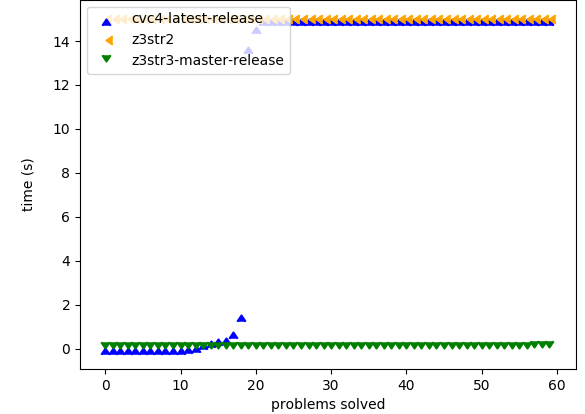
\includegraphics[width=\textwidth]{data/graphs/concats-extracts-small.png}
        \caption{Performance on \textit{Concats-Extracts-Small}}
        \label{fig:concats-extracts-small}
    \end{subfigure}
    \begin{subfigure}{.5\textwidth}
        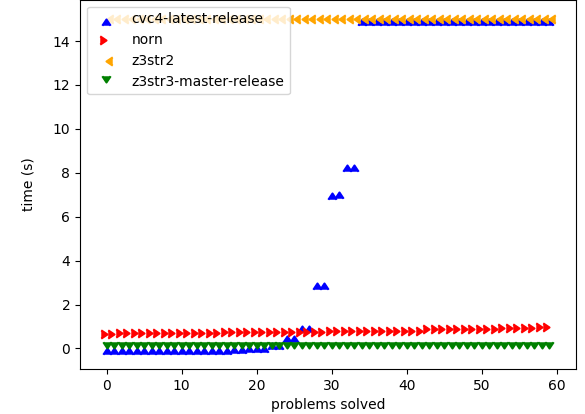
\includegraphics[width=\textwidth]{data/graphs/different-prefix.png}
        \caption{Performance on \textit{Different-Prefix}}
        \label{fig:different-prefix}
    \end{subfigure}
    \caption{Instances hard for \cvc{}}
    \label{fig:cvc-hard}

    \vspace{0.15in}

    \begin{subfigure}{.5\textwidth}
        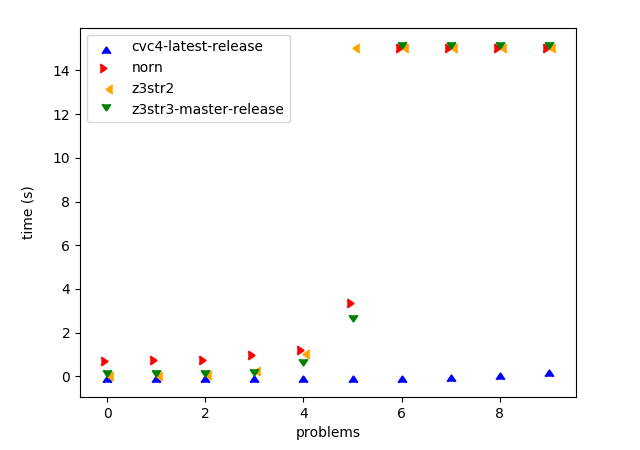
\includegraphics[width=\textwidth]{data/graphs/concats-balanced.png}
        \label{fig:concats-balanced}
        \caption{Performance on \textit{Concats-Balanced}}
    \end{subfigure}
    \begin{subfigure}{.5\textwidth}
        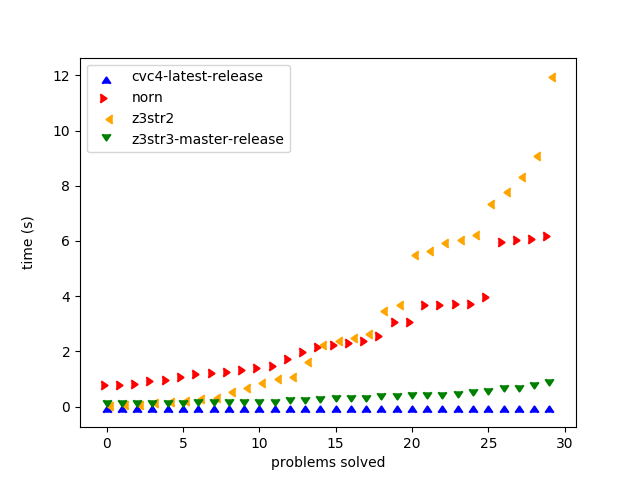
\includegraphics[width=\textwidth]{data/graphs/concats-small.png}
        \label{fig:concats-small}
        \caption{Performance on \textit{Concats-Small}}
    \end{subfigure}
    \caption{Instances hard for \us{}}
    \label{fig:z3str3-hard}
\end{figure}

\subsubsection{Usefulness to \us{}: A Case Study}

\fuzzer{}'s ability to produce scaling instances helped uncover several
implementation issues and performance limitations in \us{}. Scaling inputs
can reveal issues that would normally be out of scope for unit tests or
industrial benchmarks. Three different
performance and implementation bugs were identified and fixed in \us{}
as a result of testing with the \fuzzer{} scaling suites
\textit{Lengths} and \textit{Concats}.

\fuzzer also helped identify a number of performance-related issues and opportunities for
new heuristics in \us{}. For example, by examining \us{}'s execution traces on the
instances in the \textit{Concats} suite we discovered a
potential new heuristic. In particular, \us{} does not
make full use of the solving context (e.g. some terms are empty
strings) to simplify the concatenations of a long list of string terms
before trying to reason about the equivalences among sub-terms. \us{}
therefore introduces a large number of unnecessary intermediate
variables and propagations.
